\section{Research process}\label{sec:research-process}

The process of research conducted in the thesis is presented in Figure~\ref{fig:research-process}.
First of all, papers selected in the literature review were compared and analyzed with regard to techniques enabling the implementation of functionalities related to UIs (task 1).
The results of this analysis -- a list of concepts relevant to UI programming used by selected notations -- are introduced in subsection~\ref{sec:basis-for-evaluation} (task 2.1).

As a result of the analysis, a few descriptions (MARIA~\cite{Paterno2009, MariaPDF}, Bouchelligua et al.~\cite{Bouchelligua2010}, Kryštof~\cite{kryvstof2010lpgm}, Achilleos et al.~\cite{Achilleos2011}, and Miao et al.~\cite{Miao2017}) were excluded from the research (task 2.2) -- they were not described in enough detail to warrant an accurate evaluation of presented notations.
The exclusion did not negatively influence the research -- these papers did not provide any new concepts that were not mentioned in the included papers.
The rest of the notations (Gaouar et al.~\cite{Gaouar2018}, Khan et al.~\cite{Khan2021}, OpenUIDL~\cite{Moldovan2020}, Quid~\cite{molina2018quid, Molina2019}, Soude and Koussonda~\cite{Soude2022}, Xanui~\cite{hermida2016xanui}, Verhaeghe et al.~\cite{Verhaeghe2021visual, Verhaeghe2021behavior}) were included in the research.

Based on the results of the analysis, more rigorous evaluation criteria were defined.
The first part, presented in section~\ref{sec:evaluation-criteria}, describes the theoretical criteria for evaluating all remaining notations (task 3.1.1).
The second part (section~\ref{sec:case-study}) describes a practical experiment in which an example UI was reproduced using selected representations (task 3.2.1).

Finally, the representations were evaluated against the defined theoretical criteria (task 3.1.2).
The defined UI was also implemented (task 3.2.2) using two of the publicly available representations (OpenUIDL\furl{https://teleporthq.io/}~\cite{Moldovan2020}, Quid\furl{https://quid.metadev.pro/}~\cite{molina2018quid, Molina2019}).
The model presented by Verhaeghe et al.\furl{https://github.com/badetitou/Casino}~\cite{Verhaeghe2021visual, Verhaeghe2021behavior} was not used because the model was only available as a part of a larger project which posed a technical and logistical challenge.
The completeness of implementations was then evaluated (task 3.2.3).

\begin{figure}
    \centering
    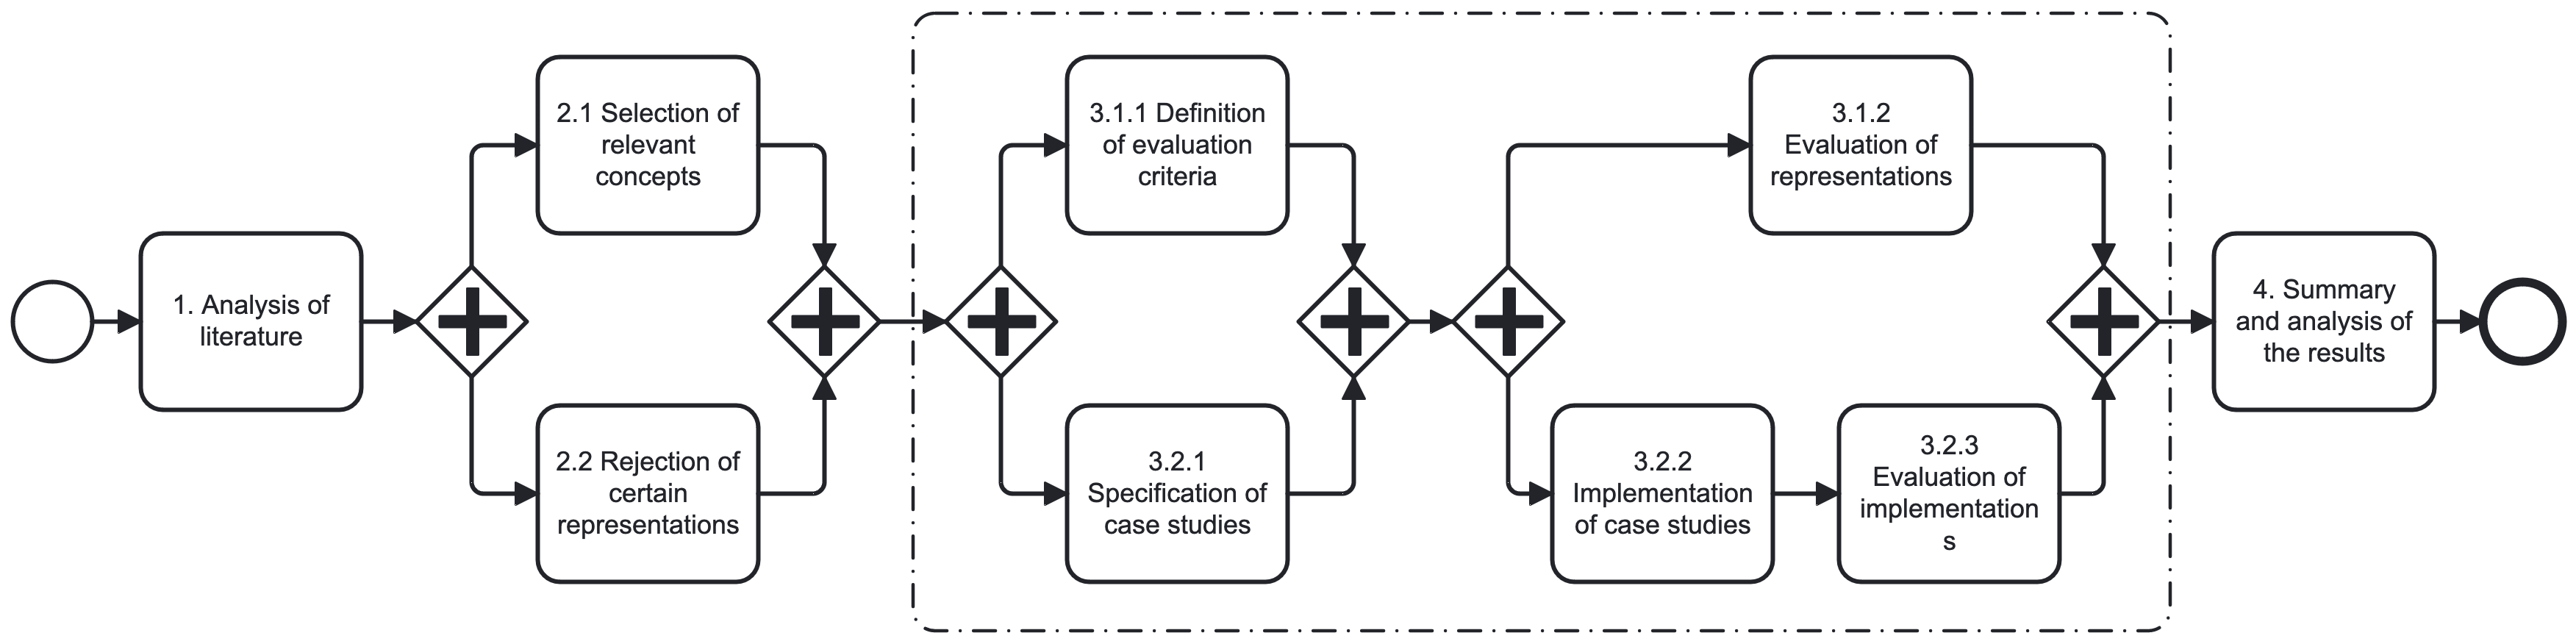
\includegraphics[width=\textwidth]{./3-research-methodology/research-process}
    \caption{BPMN diagram illustrating the research process.}
    \label{fig:research-process}
\end{figure}

The results of the evaluation and the discussion are included in the next chapter in sections~\ref{sec:results-of-evaluation} and~\ref{sec:evaluation-discussion-of-results}, respectively (task 4).
